\section{Results}
\label{sec:results}

We organize results around the four hypotheses: data efficiency (E1), grounding and its silent failure
under a flipped operator (E2/E5), mitigations (E3/E5), and compositional generalization (E4).

\subsection{E1 --- Data efficiency: integration is a large, significant win at every size}
\label{sec:e1}

\Tabref{tab:e1} and \figref{fig:data_efficiency}(a) compare the three models across six training
sizes on standard addition. The \nesy model beats the \neural baseline at \emph{every} size (all
Holm-adjusted $p{<}0.01$), tracks the oracle closely, and the gap is largest in the low-data regime.
The single most striking point is at $1{,}000$ pairs, where \nesy reaches $85.4\%$ versus the
baseline's $22.0\%$---a Cohen's $d$ of $56$ ($p{=}2.9{\times}10^{-13}$). The neural baseline needs
roughly $5{,}000$ pairs to reach what \nesy achieves with about $1{,}000$. As data grows the gap
shrinks but never closes (e.g.\ $+1.0$ point at $30{,}000$, still $p{<}0.01$), exactly the pattern the
data-efficiency claim predicts.

\begin{table}[t]
    \centering
    \resizebox{\textwidth}{!}{%
    \begin{tabular}{@{}rccccccc@{}}
        \toprule
        \textbf{\# train pairs} & \textbf{\neural} & \textbf{\nesy (sum-only)} & \textbf{\oracle}
        & \textbf{\nesy$-$\neural} & \textbf{Cohen's $d$} & \textbf{Welch $p$ (raw)}
        & \textbf{Holm-adj.\ $p$} \\
        \midrule
        100    & 0.086 & \textbf{0.130} & 0.429 & $+0.044$ & 2.28  & $8.8{\times}10^{-3}$  & $8.8{\times}10^{-3}$ \\
        500    & 0.130 & \textbf{0.649} & 0.794 & $+0.519$ & 5.43  & $9.3{\times}10^{-4}$  & $1.9{\times}10^{-3}$ \\
        1{,}000  & 0.220 & \textbf{0.854} & 0.868 & $+0.634$ & 56.3  & $2.9{\times}10^{-13}$ & $1.7{\times}10^{-12}$ \\
        5{,}000  & 0.883 & \textbf{0.955} & 0.958 & $+0.072$ & 10.25 & $1.6{\times}10^{-6}$  & $7.9{\times}10^{-6}$ \\
        15{,}000 & 0.952 & \textbf{0.973} & 0.975 & $+0.021$ & 4.82  & $3.8{\times}10^{-4}$  & $1.5{\times}10^{-3}$ \\
        30{,}000 & 0.970 & \textbf{0.980} & 0.981 & $+0.010$ & 4.13  & $4.8{\times}10^{-4}$  & $1.5{\times}10^{-3}$ \\
        \bottomrule
    \end{tabular}
    }
    \caption{\textbf{E1: data efficiency on standard addition.} Test sum accuracy (mean over $5$ seeds);
    \nesy is the sum-only neuro-symbolic model, \oracle is digit-supervised. \nesy beats the \neural
    baseline at every training size, with the largest gap at $1{,}000$ pairs ($d{=}56.3$). Every
    Holm-adjusted $p{<}0.01$, so all comparisons remain significant after family-wise correction. Best
    of \{\neural, \nesy\} in \textbf{bold}.}
    \label{tab:e1}
\end{table}


\subsection{E2 --- Grounding emerges without any digit labels (standard addition)}
\label{sec:e2}

\figref{fig:data_efficiency}(b) shows that \nesy's latent digit-grounding rises from $28.3\%$
(100 pairs) to $99.0\%$ ($30$k pairs), essentially matching the digit-supervised oracle---even though
\nesy never saw a digit label. The Hungarian-aligned grounding \emph{equals} the raw grounding at every
size ($0/5$ shortcut flags throughout), so standard \mnistadd is \newterm{shortcut-robust}: its boundary
sums uniquely pin the symbols. The visible sum-vs-grounding gap (e.g.\ $85.4\%$ sum vs.\ $92.4\%$
grounding at $1$k) is just the ``both digits must be right'' effect (sum~$\approx$~grounding$^2$), not a
shortcut.

\begin{figure}[t]
    \centering
    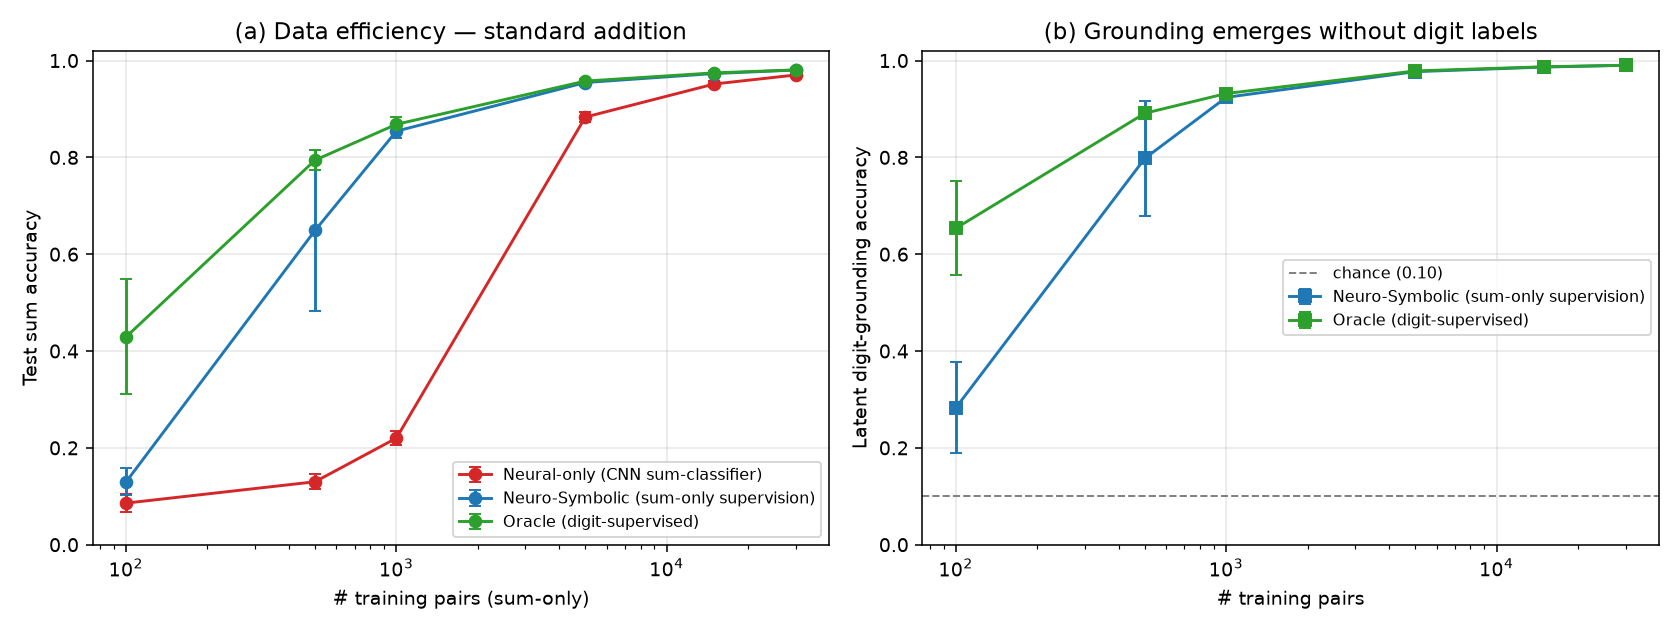
\includegraphics[width=0.95\linewidth]{figures/fig1_data_efficiency.png}
    \caption{\figleft Data efficiency on standard addition. \nesy (blue) dramatically beats the
    \neural baseline (red), most sharply in the low-data regime, and tracks the digit-supervised oracle
    (green); the baseline needs ${\sim}5{\times}$ more data to catch up. \figright Latent
    digit-grounding accuracy rises to $99\%$ for \nesy with \emph{no} digit labels, matching the oracle
    and far above the $0.10$ chance line. Error bars are $95\%$ confidence intervals over $5$ seeds.}
    \label{fig:data_efficiency}
\end{figure}

\subsection{E5 --- Flip the operator and grounding collapses}
\label{sec:e5}

Changing \emph{only} the symbolic operator to \modten produces a sharp dissociation between task
accuracy and grounding (\Tabref{tab:e5}, \twofigref{fig:shortcut}{fig:confusion}). Standard addition
grounds at $99.0\%$; modular addition grounds at $\approx2\%$ raw. Among the four seeds that actually
learn the modular task (sum${>}0.3$), raw grounding is just $0.09\%$ (max $0.16\%$): the network reads
the digits systematically wrong via a global relabeling that leaves \modten invariant. The
permutation-aligned metric makes the failure legible---aligned grounding is $0.53$--$0.60$ on shortcut
seeds and reaches $0.99$ on the cleanest realization, where the model lands on the \emph{exact}
predicted cyclic shift $d\mapsto(d{+}5)\bmod 10$ (\figref{fig:confusion}). The fifth seed collapses to
predicting a single class. Crucially, the digit-supervised \emph{oracle grounds at $99.0\%$ on the
identical modular task}, so the collapse is caused by distant supervision under a symmetric operator,
not by the task. The standard-vs-modular grounding contrast is overwhelming ($0.990$ vs.\ $0.020$,
Welch $p{=}9.6{\times}10^{-7}$, $d{=}31.5$). This shortcut is visible \emph{only} because we measured
grounding; task accuracy alone is blind to it.

\begin{table}[t]
    \centering
    \resizebox{\textwidth}{!}{%
    \begin{tabular}{@{}lcccl@{}}
        \toprule
        \textbf{Task (\nesy, $N{=}30$k)} & \textbf{Sum acc (mean${\pm}$CI)} & \textbf{Grounding (raw)}
        & \textbf{Hungarian-aligned} & \textbf{Outcome over $5$ seeds} \\
        \midrule
        standard $a{+}b$ & $0.980 \pm 0.002$ & \textbf{0.990} & 0.990 & $0/5$ shortcut (grounds correctly) \\
        modular \modten & $0.657 \pm 0.380$ & \textbf{0.020} & 0.471 & \textbf{$4/5$ shortcut $+$ $1/5$ collapse} \\
        modular --- \oracle (digit-sup.) & 0.979 & \textbf{0.990} & 0.990 & $0/5$ (control: same task, grounds fine) \\
        \bottomrule
    \end{tabular}
    }
    \caption{\textbf{E5: flipping the operator switches shortcuts on.} Changing only $a{+}b\to\modten$
    leaves task accuracy non-trivial but collapses raw grounding from $0.990$ to $0.020$; the large
    aligned${-}$raw gap reveals a systematic relabeling. The digit-supervised oracle grounds at $0.990$
    on the \emph{same} modular task (control), so the failure is caused by distant supervision under a
    symmetric operator. Standard vs.\ modular grounding: Welch $p{=}9.6{\times}10^{-7}$, $d{=}31.5$.}
    \label{tab:e5}
\end{table}


\begin{figure}[t]
    \centering
    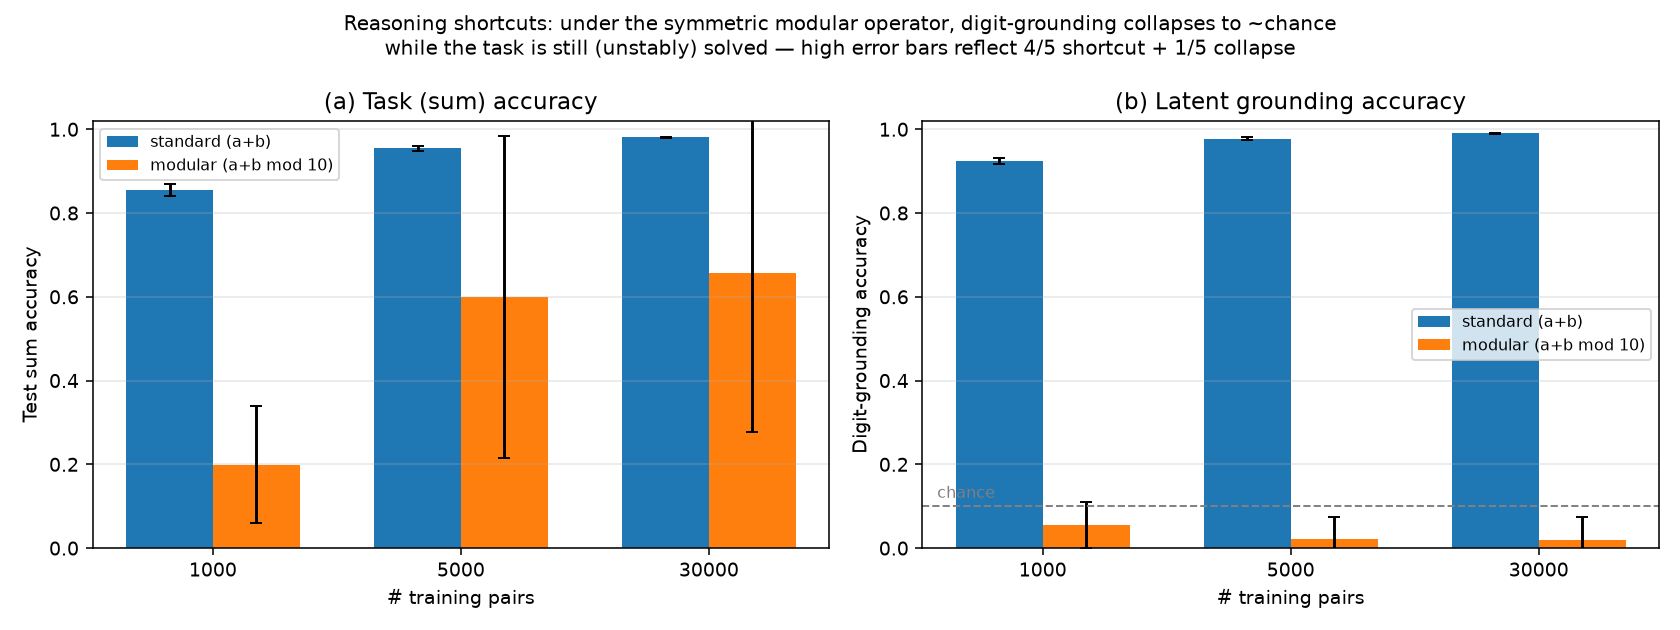
\includegraphics[width=0.95\linewidth]{figures/fig2_shortcut.png}
    \caption{Flipping one operator switches reasoning shortcuts on. \figleft Task (sum) accuracy:
    standard addition (blue) is high and stable, while modular addition (orange) is solved
    \emph{unstably}---the large error bars reflect $4/5$ seeds finding a shortcut and $1/5$ collapsing.
    \figright Latent grounding: standard addition reaches $99\%$, but modular addition sits near the
    $0.10$ chance line---high task accuracy with near-zero grounding. Bars are means over $5$ seeds;
    error bars are $95\%$ confidence intervals.}
    \label{fig:shortcut}
\end{figure}

\begin{figure}[t]
    \centering
    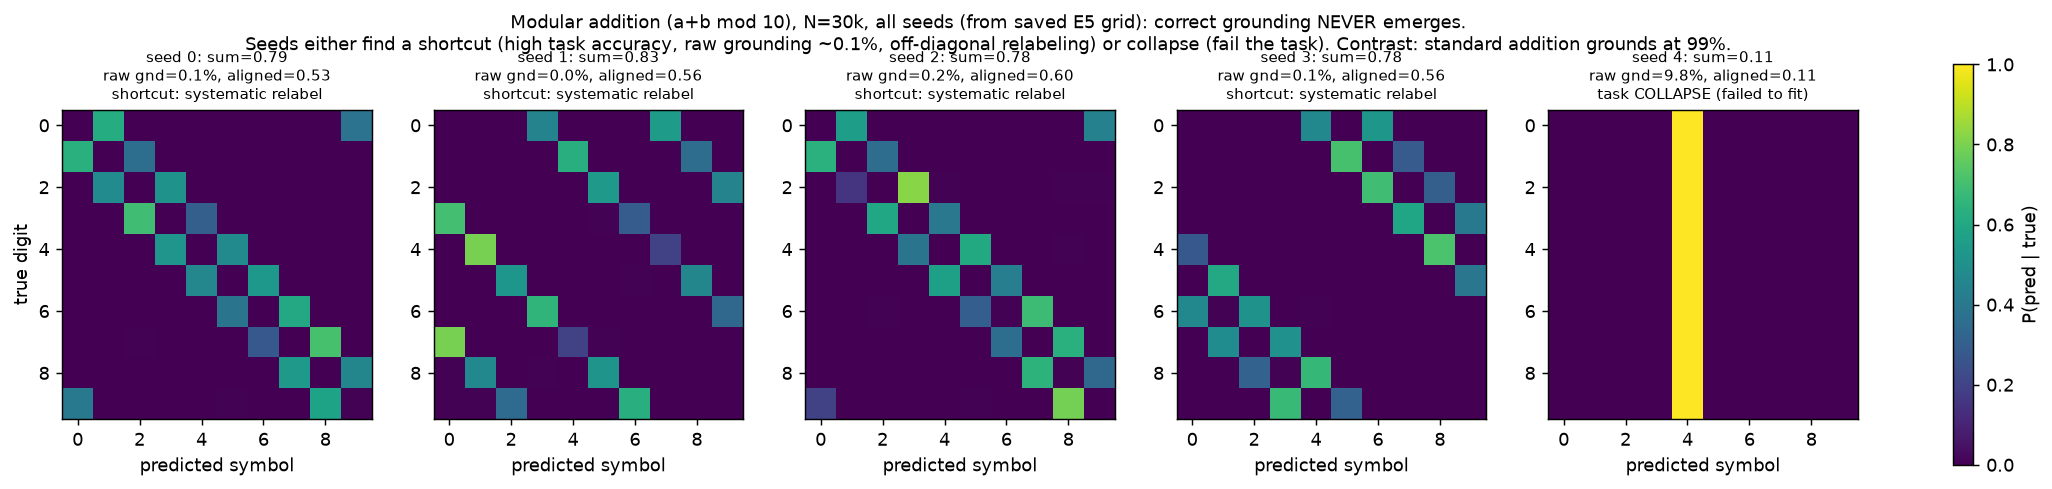
\includegraphics[width=0.98\linewidth]{figures/fig3_confusion.png}
    \caption{Per-seed grounding confusion matrices (rows: true digit, columns: predicted symbol) for
    modular addition at $N{=}30$k, read from the saved E5 grid. Seeds 0--3 place nearly all mass
    \emph{off} the diagonal: a clean, systematic relabeling (a reasoning shortcut) rather than random
    noise---seed 1 is close to the exact $d\mapsto(d{+}5)$ cyclic shift. Seed 4 collapses to a single
    predicted class (failed to fit). Correct grounding never appears, whereas standard addition grounds
    on the diagonal at $99\%$.}
    \label{fig:confusion}
\end{figure}

\subsection{E3/E5 --- Mitigations: needed and effective exactly when a shortcut exists}
\label{sec:e3}

\Tabref{tab:e3} and \figref{fig:mitigations} report grounding accuracy under each intervention. We
evaluate standard addition at $N{=}1$k (where its grounding gap is largest) and modular addition at
$N{=}5$k (where the shortcut is firmly established); each column is a within-task before/after
comparison, so the differing $N$ does not affect the conclusion. On standard addition, where there is no
shortcut to fix, mitigations do essentially nothing. On modular addition, \emph{just $10$ labeled
images} (one per class) break the symmetry and restore grounding from $\approx0.1\%$ to $97.7\%$ in
\emph{every} seed (per-seed $0.973$--$0.981$; Welch $p{=}1.6{\times}10^{-3}$, $d{=}4.8$), while also
stabilizing training (sum accuracy $\to0.954$, no collapses). Adding more labels ($50$, $200$) does not
help further. Unsupervised regularizers are unreliable: a marginal-uniformity prior recovers only
partial grounding ($0.390$, high variance) and an entropy penalty does not help at all ($0.128$). The
cure matches the disease---supply the missing identifying constraint---and it is extremely cheap.

\begin{table}[t]
    \centering
    \begin{tabular}{@{}lcc@{}}
        \toprule
        \textbf{Intervention} & \textbf{Standard add @$N{=}1$k} & \textbf{Modular add @$N{=}5$k} \\
         & \textbf{(no shortcut)} & \textbf{(shortcut present)} \\
        \midrule
        baseline (none)                              & 0.924 & 0.116 \footnotesize{(4/5 $\approx$0; 1 seed 0.57)} \\
        $+$ aux digit labels, 1/class (10 total)     & 0.925 & \textbf{0.977} \\
        $+$ aux 5/class (50 total)                   & 0.926 & 0.977 \\
        $+$ aux 20/class (200 total)                 & 0.931 & 0.979 \\
        $+$ marginal-uniformity prior                & 0.924 & 0.390 \\
        $+$ entropy regularization                   & 0.925 & 0.128 \\
        \bottomrule
    \end{tabular}
    \caption{\textbf{E3: mitigations restore grounding only when a shortcut exists.} Digit-grounding
    accuracy under each intervention (standard addition evaluated at $N{=}1$k, modular at $N{=}5$k; each
    column is a within-task before/after). On standard addition there is nothing to fix. On modular
    addition, just $10$ labeled images break the symmetry and restore grounding to $0.977$ in every seed
    (Welch $p{=}1.6{\times}10^{-3}$, $d{=}4.8$), whereas unsupervised regularizers help only partially
    (uniform prior) or not at all (entropy). Best modular result in \textbf{bold}.}
    \label{tab:e3}
\end{table}


\begin{figure}[t]
    \centering
    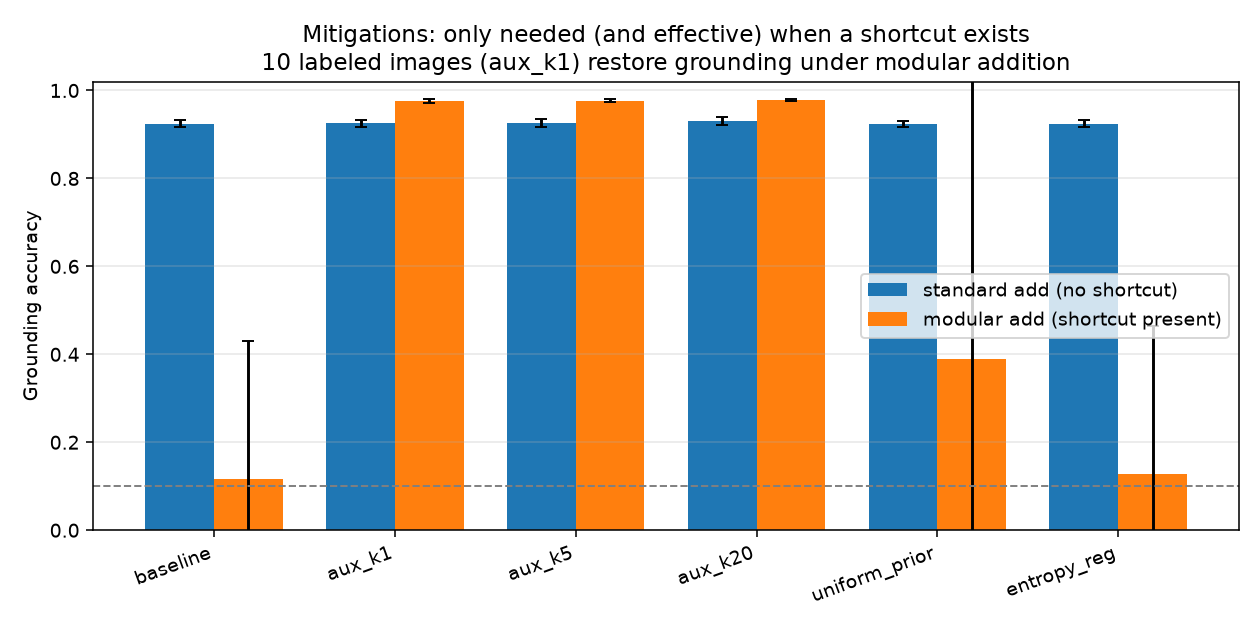
\includegraphics[width=0.85\linewidth]{figures/fig5_mitigations.png}
    \caption{Mitigations are needed (and effective) only when a shortcut exists. On standard addition
    (blue, no shortcut) all interventions leave grounding essentially unchanged. On modular addition
    (orange, shortcut present) just $10$ labeled images (\texttt{aux\_k1}) restore grounding to
    $97.7\%$; more labels add nothing, the uniform prior helps only partially (high variance), and the
    entropy penalty does not help. Dashed line is the $0.10$ chance level.}
    \label{fig:mitigations}
\end{figure}

\subsection{E4 --- Compositional generalization: the payoff of correct grounding}
\label{sec:e4}

Finally, \Tabref{tab:e4} and \figref{fig:ood} show the capability that correct grounding unlocks.
Trained on \emph{single-digit} sums only, the \nesy model solves $2$- and $3$-digit number addition it
never saw---at $95.7\%$ and $93.7\%$---by composing its digit classifier with a symbolic place-value
sum, essentially matching the oracle ($96.0\%$/$94.0\%$). The \neural baseline scores exactly $0\%$: it
cannot even emit sums in this range, a structural rather than a tuning failure. Across the grounded
models, single-digit grounding and OOD accuracy correlate almost perfectly (Pearson $r{=}0.993$,
$p{=}1{\times}10^{-8}$), but because that correlation spans models that all ground well, we treat the
\emph{categorical} contrast ($0\%$ for the ungrounded baseline vs.\ ${\sim}96\%$ for grounded models) as
the stronger evidence. This is the most direct demonstration that integration buys a genuinely new
capability, not just a higher benchmark number---and that the capability rests on correct grounding.

\begin{table}[t]
    \centering
    \begin{tabular}{@{}lccc@{}}
        \toprule
        \textbf{Model} & \textbf{2-digit (OOD)} & \textbf{3-digit (OOD)} & \textbf{single-digit grounding} \\
        \midrule
        \neural          & 0.000 & 0.000 & 0.000 (n/a) \\
        \nesy            & \textbf{0.957} & \textbf{0.937} & 0.990 \\
        \oracle          & 0.960 & 0.940 & 0.990 \\
        \bottomrule
    \end{tabular}
    \caption{\textbf{E4: compositional generalization.} Models trained only on single-digit sums,
    evaluated zero-shot on multi-digit number addition via symbolic place-value composition. \nesy nearly
    matches the oracle and generalizes to a structure it never saw, \emph{because} its grounding is
    correct; the \neural baseline cannot represent outputs in this range (structural $0\%$). Best of the
    two learnable contrasts (\neural, \nesy) in \textbf{bold}.}
    \label{tab:e4}
\end{table}


\begin{figure}[t]
    \centering
    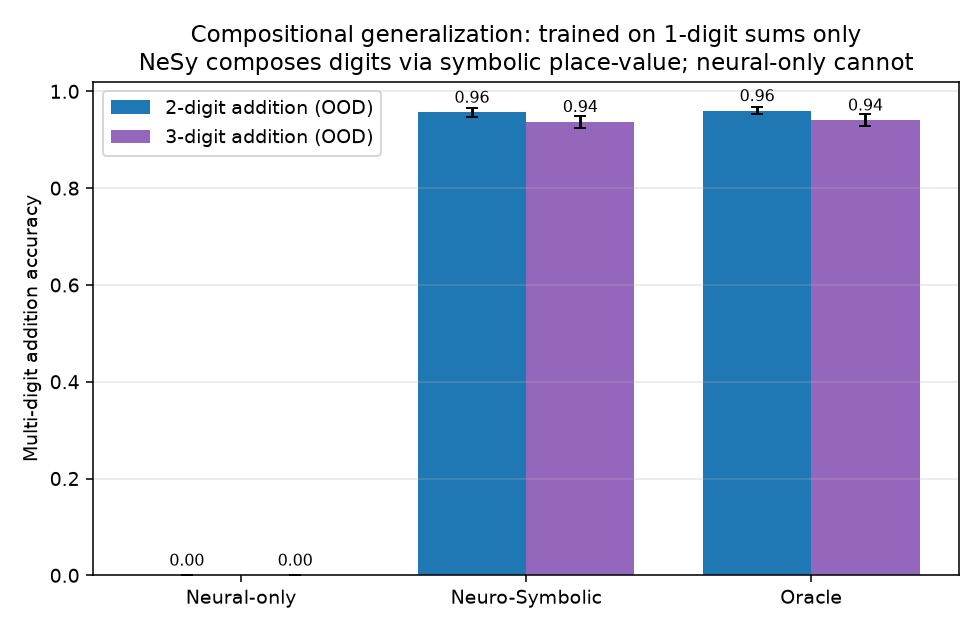
\includegraphics[width=0.7\linewidth]{figures/fig4_compositional_ood.png}
    \caption{Zero-shot compositional generalization. Trained only on single-digit sums, \nesy and the
    oracle solve $2$- and $3$-digit number addition at ${\sim}94$--$96\%$ by composing the digit
    classifier with a symbolic place-value sum. The \neural baseline scores $0\%$---it structurally
    cannot represent outputs in this range. Error bars are $95\%$ confidence intervals over $5$ seeds.}
    \label{fig:ood}
\end{figure}
